% Options for packages loaded elsewhere
\PassOptionsToPackage{unicode}{hyperref}
\PassOptionsToPackage{hyphens}{url}
\documentclass[
]{article}
\usepackage{xcolor}
\usepackage[margin=1in]{geometry}
\usepackage{amsmath,amssymb}
\setcounter{secnumdepth}{-\maxdimen} % remove section numbering
\usepackage{iftex}
\ifPDFTeX
  \usepackage[T1]{fontenc}
  \usepackage[utf8]{inputenc}
  \usepackage{textcomp} % provide euro and other symbols
\else % if luatex or xetex
  \usepackage{unicode-math} % this also loads fontspec
  \defaultfontfeatures{Scale=MatchLowercase}
  \defaultfontfeatures[\rmfamily]{Ligatures=TeX,Scale=1}
\fi
\usepackage{lmodern}
\ifPDFTeX\else
  % xetex/luatex font selection
\fi
% Use upquote if available, for straight quotes in verbatim environments
\IfFileExists{upquote.sty}{\usepackage{upquote}}{}
\IfFileExists{microtype.sty}{% use microtype if available
  \usepackage[]{microtype}
  \UseMicrotypeSet[protrusion]{basicmath} % disable protrusion for tt fonts
}{}
\makeatletter
\@ifundefined{KOMAClassName}{% if non-KOMA class
  \IfFileExists{parskip.sty}{%
    \usepackage{parskip}
  }{% else
    \setlength{\parindent}{0pt}
    \setlength{\parskip}{6pt plus 2pt minus 1pt}}
}{% if KOMA class
  \KOMAoptions{parskip=half}}
\makeatother
\usepackage{color}
\usepackage{fancyvrb}
\newcommand{\VerbBar}{|}
\newcommand{\VERB}{\Verb[commandchars=\\\{\}]}
\DefineVerbatimEnvironment{Highlighting}{Verbatim}{commandchars=\\\{\}}
% Add ',fontsize=\small' for more characters per line
\usepackage{framed}
\definecolor{shadecolor}{RGB}{248,248,248}
\newenvironment{Shaded}{\begin{snugshade}}{\end{snugshade}}
\newcommand{\AlertTok}[1]{\textcolor[rgb]{0.94,0.16,0.16}{#1}}
\newcommand{\AnnotationTok}[1]{\textcolor[rgb]{0.56,0.35,0.01}{\textbf{\textit{#1}}}}
\newcommand{\AttributeTok}[1]{\textcolor[rgb]{0.13,0.29,0.53}{#1}}
\newcommand{\BaseNTok}[1]{\textcolor[rgb]{0.00,0.00,0.81}{#1}}
\newcommand{\BuiltInTok}[1]{#1}
\newcommand{\CharTok}[1]{\textcolor[rgb]{0.31,0.60,0.02}{#1}}
\newcommand{\CommentTok}[1]{\textcolor[rgb]{0.56,0.35,0.01}{\textit{#1}}}
\newcommand{\CommentVarTok}[1]{\textcolor[rgb]{0.56,0.35,0.01}{\textbf{\textit{#1}}}}
\newcommand{\ConstantTok}[1]{\textcolor[rgb]{0.56,0.35,0.01}{#1}}
\newcommand{\ControlFlowTok}[1]{\textcolor[rgb]{0.13,0.29,0.53}{\textbf{#1}}}
\newcommand{\DataTypeTok}[1]{\textcolor[rgb]{0.13,0.29,0.53}{#1}}
\newcommand{\DecValTok}[1]{\textcolor[rgb]{0.00,0.00,0.81}{#1}}
\newcommand{\DocumentationTok}[1]{\textcolor[rgb]{0.56,0.35,0.01}{\textbf{\textit{#1}}}}
\newcommand{\ErrorTok}[1]{\textcolor[rgb]{0.64,0.00,0.00}{\textbf{#1}}}
\newcommand{\ExtensionTok}[1]{#1}
\newcommand{\FloatTok}[1]{\textcolor[rgb]{0.00,0.00,0.81}{#1}}
\newcommand{\FunctionTok}[1]{\textcolor[rgb]{0.13,0.29,0.53}{\textbf{#1}}}
\newcommand{\ImportTok}[1]{#1}
\newcommand{\InformationTok}[1]{\textcolor[rgb]{0.56,0.35,0.01}{\textbf{\textit{#1}}}}
\newcommand{\KeywordTok}[1]{\textcolor[rgb]{0.13,0.29,0.53}{\textbf{#1}}}
\newcommand{\NormalTok}[1]{#1}
\newcommand{\OperatorTok}[1]{\textcolor[rgb]{0.81,0.36,0.00}{\textbf{#1}}}
\newcommand{\OtherTok}[1]{\textcolor[rgb]{0.56,0.35,0.01}{#1}}
\newcommand{\PreprocessorTok}[1]{\textcolor[rgb]{0.56,0.35,0.01}{\textit{#1}}}
\newcommand{\RegionMarkerTok}[1]{#1}
\newcommand{\SpecialCharTok}[1]{\textcolor[rgb]{0.81,0.36,0.00}{\textbf{#1}}}
\newcommand{\SpecialStringTok}[1]{\textcolor[rgb]{0.31,0.60,0.02}{#1}}
\newcommand{\StringTok}[1]{\textcolor[rgb]{0.31,0.60,0.02}{#1}}
\newcommand{\VariableTok}[1]{\textcolor[rgb]{0.00,0.00,0.00}{#1}}
\newcommand{\VerbatimStringTok}[1]{\textcolor[rgb]{0.31,0.60,0.02}{#1}}
\newcommand{\WarningTok}[1]{\textcolor[rgb]{0.56,0.35,0.01}{\textbf{\textit{#1}}}}
\usepackage{graphicx}
\makeatletter
\newsavebox\pandoc@box
\newcommand*\pandocbounded[1]{% scales image to fit in text height/width
  \sbox\pandoc@box{#1}%
  \Gscale@div\@tempa{\textheight}{\dimexpr\ht\pandoc@box+\dp\pandoc@box\relax}%
  \Gscale@div\@tempb{\linewidth}{\wd\pandoc@box}%
  \ifdim\@tempb\p@<\@tempa\p@\let\@tempa\@tempb\fi% select the smaller of both
  \ifdim\@tempa\p@<\p@\scalebox{\@tempa}{\usebox\pandoc@box}%
  \else\usebox{\pandoc@box}%
  \fi%
}
% Set default figure placement to htbp
\def\fps@figure{htbp}
\makeatother
\setlength{\emergencystretch}{3em} % prevent overfull lines
\providecommand{\tightlist}{%
  \setlength{\itemsep}{0pt}\setlength{\parskip}{0pt}}
\usepackage{hyperref}
\usepackage{amsmath}
\usepackage{amssymb}
\usepackage{graphicx}
\usepackage{fontspec}
\usepackage{xcolor}
\usepackage{tikz}
\definecolor{blue}{RGB}{0, 100, 0}
\setmainfont{Times New Roman}
\setsansfont{Times New Roman}
\setmonofont{Courier New}
\usepackage[margin=1in]{geometry}
\usepackage{titlesec}
\titleformat{\section}{\Huge\bfseries\color{pink}}{\thesection}{1em}{}
\titleformat{\subsection}{\huge\bfseries\color{pink}}{\thesubsection}{1em}{}
\titleformat{\subsubsection}{\LARGE\bfseries\color{pink}}{\thesubsubsection}{1em}{}
\usepackage{tocloft}
\renewcommand{\cftsecfont}{\small}
\renewcommand{\cftsubsecfont}{\footnotesize}
\renewcommand{\cftsecpagefont}{\small}
\renewcommand{\cftsubsecpagefont}{\footnotesize}
\renewcommand{\cftsecleader}{\cftdotfill{\cftdotsep}}
\usepackage{booktabs}
\usepackage{caption}
\usepackage{longtable}
\usepackage{colortbl}
\usepackage{array}
\usepackage{anyfontsize}
\usepackage{multirow}
\usepackage{bookmark}
\IfFileExists{xurl.sty}{\usepackage{xurl}}{} % add URL line breaks if available
\urlstyle{same}
\hypersetup{
  hidelinks,
  pdfcreator={LaTeX via pandoc}}

\author{}
\date{\vspace{-2.5em}}

\begin{document}

\begin{titlepage}
    \begin{center}
    % Début de la bordure avec TikZ
    \begin{tikzpicture}[remember picture, overlay] % overlay = force TikZ à dessiner par-dessus le contenu existant de la page, plutôt que de réserver un espace supplémentaire pour le dessin, remember = lorsque vous voulez dessiner par rapport à la position exacte de la page
    % Définir une couleur élégante
    \definecolor{blue}{RGB}{0, 100, 0}
    
    % Dessiner une bordure élégante avec coins arrondis
    \draw[
        line width=5pt, % Épaisseur du trait
        pink, % Couleur de la bordure
        rounded corners=15pt, % Coins arrondis
        double, % Bordure double
        double distance=2pt % Espacement entre les deux lignes
    ] 
        ([xshift=10pt, yshift=-10pt]current page.north west) rectangle
        ([xshift=-10pt, yshift=10pt]current page.south east);
    \end{tikzpicture}
        
\includegraphics[width=7cm]{Figures/LOGO1.jpeg} \\[0.1cm]  % C:/Users/hp/Desktop/AwaDIAW_ISE-CL/Semestre2/Informatique/Projet_Statistique_avec_R/Tps_sem6
        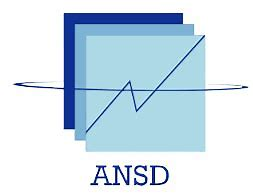
\includegraphics[width=6cm]{Figures/LOGO2.jpeg} \\[0.1cm] % C:/Users/hp/Desktop/AwaDIAW_ISE-CL/Semestre2/Informatique/Projet_Statistique_avec_R/Tps_sem6
        
        \textbf{\large Agence nationale de la Statistique et de la Démographie (ANSD)}\\[0.2cm]
        
        
\includegraphics[width=4cm]{Figures/LOGO3.jpeg} \\[0.1cm]  % C:/Users/hp/Desktop/AwaDIAW_ISE-CL/Semestre2/Informatique/Projet_Statistique_avec_R/Tps_sem6
        
        \textbf{\large Ecole nationale de la Statistique et de l'Analyse économique Pierre Ndiaye (ENSAE)}\\[0.4cm]
        
        \textit{\LARGE Semestre 2 : Projet statistique sous R }\\[0.3cm]
        \textbf{\Huge \color{blue} \textsf{Statistiques descriptives avec gtsummary}}\\[0.2cm]
        
        \begin{minipage}{0.5\textwidth}
    \begin{flushleft} \large
        \emph{\textsf{Rédigé par :}}\\
        \textbf{Khadidiatou Diakhaté}\\
        \textit{Elève en ISEP3}
    \end{flushleft}
\end{minipage}
        \hfill
        \begin{minipage}{0.4\textwidth}
            \begin{flushright} \large
                \emph{\textsf{Sous la supervision de :}} \\
                \textbf{M. Aboubacre HEMA}\\
                \textit{Research Analyst }
            \end{flushright}
        \end{minipage}

        \vfill 

        {\large \textsf{Année scolaire : 2024/2025}}\\[0.5cm]
        
    \end{center}
\end{titlepage}

\subsection{Installation des packages si
nécessaire}\label{installation-des-packages-si-nuxe9cessaire}

\begin{Shaded}
\begin{Highlighting}[]
\NormalTok{packages }\OtherTok{\textless{}{-}} \FunctionTok{c}\NormalTok{(}\StringTok{"haven"}\NormalTok{,}\StringTok{"dplyr"}\NormalTok{,}\StringTok{"gtsummary"}\NormalTok{,}\StringTok{"labelled"}\NormalTok{)}


\ControlFlowTok{for}\NormalTok{ (package }\ControlFlowTok{in}\NormalTok{ packages) \{}
  \ControlFlowTok{if}\NormalTok{ (}\SpecialCharTok{!}\FunctionTok{requireNamespace}\NormalTok{(package, }\AttributeTok{quietly =} \ConstantTok{TRUE}\NormalTok{)) \{   }\CommentTok{\# Vérifie si le package n\textquotesingle{}est pas encore installé}
    \FunctionTok{install.packages}\NormalTok{(package)}
\NormalTok{  \}}
  \FunctionTok{library}\NormalTok{(package, }\AttributeTok{character.only =} \ConstantTok{TRUE}\NormalTok{) }\CommentTok{\# nom du package en nom ou chaine de caractère ()}
\NormalTok{\}}
\end{Highlighting}
\end{Shaded}

\subsection{Exportation des bases}\label{exportation-des-bases}

\begin{Shaded}
\begin{Highlighting}[]
\FunctionTok{library}\NormalTok{(haven)}
\NormalTok{ehcvm\_menage }\OtherTok{\textless{}{-}} \FunctionTok{read\_dta}\NormalTok{(}\StringTok{"donnees/ehcvm\_menage\_gnb2021.dta"}\NormalTok{) }\CommentTok{\# qui concerne les caractéristiques du ménage}
\NormalTok{ehcvm\_welfare }\OtherTok{\textless{}{-}} \FunctionTok{read\_dta}\NormalTok{(}\StringTok{"donnees/ehcvm\_welfare\_gnb2021.dta"}\NormalTok{) }\CommentTok{\# qui concerne le bien{-}être du ménage}
\CommentTok{\#Visualisons quelques observations de ces bases}
\FunctionTok{head}\NormalTok{(ehcvm\_menage)}
\end{Highlighting}
\end{Shaded}

\begin{verbatim}
## # A tibble: 6 x 38
##   country     hhid  year grappe menage vague logem     mur  toit   sol eauboi_ss
##   <chr>      <dbl> <dbl>  <dbl>  <dbl> <dbl> <dbl+l> <dbl> <dbl> <dbl>     <dbl>
## 1 GNB     11122701  2021 111227      1     1 2 [Pro~     1     0     0         1
## 2 GNB     11122702  2021 111227      2     1 2 [Pro~     0     1     0         0
## 3 GNB     11122703  2021 111227      3     1 2 [Pro~     0     1     0         0
## 4 GNB     11122704  2021 111227      4     1 2 [Pro~     0     0     0         0
## 5 GNB     11122705  2021 111227      5     1 2 [Pro~     1     0     0         1
## 6 GNB     11122708  2021 111227      8     1 2 [Pro~     0     1     1         1
## # i 27 more variables: eauboi_sp <dbl>, elec_ac <dbl>, elec_ur <dbl>,
## #   elec_ua <dbl>, ordure <dbl>, toilet <dbl>, eva_toi <dbl>, eva_eau <dbl>,
## #   tv <dbl>, fer <dbl>, frigo <dbl>, cuisin <dbl>, ordin <dbl>, decod <dbl>,
## #   car <dbl>, superf <dbl>, grosrum <dbl>, petitrum <dbl>, porc <dbl>,
## #   lapin <dbl>, volail <dbl>, sh_id_demo <dbl>, sh_co_natu <dbl>,
## #   sh_co_eco <dbl>, sh_id_eco <dbl>, sh_co_vio <dbl>, sh_co_oth <dbl>
\end{verbatim}

\begin{Shaded}
\begin{Highlighting}[]
\FunctionTok{head}\NormalTok{(ehcvm\_welfare)}
\end{Highlighting}
\end{Shaded}

\begin{verbatim}
## # A tibble: 6 x 43
##   grappe menage country  year      hhid vague month      zae     region  milieu 
##    <dbl>  <dbl> <chr>   <dbl>     <dbl> <dbl> <date>     <dbl+l> <dbl+l> <dbl+l>
## 1 111227     11 GNB      2021 111227011     1 2021-12-01 7 [Zon~ 1 [Tom~ 2 [Rur~
## 2 111227     46 GNB      2021 111227046     1 2021-12-01 7 [Zon~ 1 [Tom~ 2 [Rur~
## 3 111227      2 GNB      2021  11122702     1 2021-12-01 7 [Zon~ 1 [Tom~ 2 [Rur~
## 4 111227     13 GNB      2021 111227013     1 2021-12-01 7 [Zon~ 1 [Tom~ 2 [Rur~
## 5 111227      3 GNB      2021  11122703     1 2021-12-01 7 [Zon~ 1 [Tom~ 2 [Rur~
## 6 111227     10 GNB      2021 111227010     1 2021-12-01 7 [Zon~ 1 [Tom~ 2 [Rur~
## # i 33 more variables: hhweight <dbl>, hhsize <dbl>, eqadu1 <dbl>,
## #   eqadu2 <dbl>, hgender <dbl+lbl>, hage <dbl>, hmstat <dbl+lbl>,
## #   hreligion <dbl+lbl>, hnation <dbl+lbl>, hethnie <dbl+lbl>, halfa <dbl+lbl>,
## #   halfa2 <dbl+lbl>, heduc <dbl+lbl>, hdiploma <dbl+lbl>, hhandig <dbl+lbl>,
## #   hactiv7j <dbl+lbl>, hactiv12m <dbl+lbl>, hbranch <dbl+lbl>,
## #   hsectins <dbl+lbl>, hcsp <dbl+lbl>, dali <dbl>, dnal <dbl>, dtot <dbl>,
## #   pcexp <dbl>, zref <dbl>, def_spa <dbl>, def_temp <dbl>, ...
\end{verbatim}

\subsection{Réalisation pas-à pas d'un tableau avec le package
gtsummary}\label{ruxe9alisation-pas-uxe0-pas-dun-tableau-avec-le-package-gtsummary}

Avec la base ehcvm\_menage, nous allons présenter quelques statistiques
descriptives des variables logem(logement), toit(type de toit), mur(type
de mur) et sol(type de sol). Utilisons \textbf{tbl\_summary} pour cela :

\begin{Shaded}
\begin{Highlighting}[]
\FunctionTok{library}\NormalTok{(gtsummary)}
\NormalTok{ehcvm\_menage }\SpecialCharTok{\%\textgreater{}\%} \FunctionTok{select}\NormalTok{(logem,mur,toit,sol) }\SpecialCharTok{\%\textgreater{}\%} \FunctionTok{tbl\_summary}\NormalTok{()}
\end{Highlighting}
\end{Shaded}

\begin{verbatim}
## ! Column(s) "logem" are class "haven_labelled".
## i This is an intermediate datastructure not meant for analysis.
## i Convert columns with `haven::as_factor()`, `labelled::to_factor()`,
##   `labelled::unlabelled()`, and `unclass()`. Failure to convert may have
##   unintended consequences or result in error.
## <https://haven.tidyverse.org/articles/semantics.html>
## <https://larmarange.github.io/labelled/articles/intro_labelled.html#unlabelled>
\end{verbatim}

\begin{table}[!t]
\fontsize{12.0pt}{14.4pt}\selectfont
\begin{tabular*}{\linewidth}{@{\extracolsep{\fill}}lc}
\toprule
\textbf{Characteristic} & \textbf{N = 5,351}\textsuperscript{\textit{1}} \\ 
\midrule\addlinespace[2.5pt]
Ocupaçao de alojamento &  \\ 
    1 & 1,263 (24\%) \\ 
    2 & 3,095 (58\%) \\ 
    3 & 574 (11\%) \\ 
    4 & 419 (7.8\%) \\ 
Parede em materiais definitivos & 1,619 (30\%) \\ 
Tecto em materiais definitivos & 4,586 (86\%) \\ 
Solo em materiais definitivos & 2,737 (51\%) \\ 
\bottomrule
\end{tabular*}
\begin{minipage}{\linewidth}
\textsuperscript{\textit{1}}n (\%)\\
\end{minipage}
\end{table}

Cependant, avec ce tableau, on ne voit pas les labels des modalités des
variables. Pour les afficher, on va utiliser la fonction
\textbf{to\_factor() du package labelled}.

\begin{Shaded}
\begin{Highlighting}[]
\FunctionTok{library}\NormalTok{(labelled)}
\NormalTok{ehcvm\_menage }\SpecialCharTok{\%\textgreater{}\%}\NormalTok{ labelled}\SpecialCharTok{::}\FunctionTok{to\_factor}\NormalTok{() }\SpecialCharTok{\%\textgreater{}\%}\FunctionTok{select}\NormalTok{(logem,mur,toit,sol) }\SpecialCharTok{\%\textgreater{}\%} \FunctionTok{tbl\_summary}\NormalTok{()}
\end{Highlighting}
\end{Shaded}

\begin{table}[!t]
\fontsize{12.0pt}{14.4pt}\selectfont
\begin{tabular*}{\linewidth}{@{\extracolsep{\fill}}lc}
\toprule
\textbf{Characteristic} & \textbf{N = 5,351}\textsuperscript{\textit{1}} \\ 
\midrule\addlinespace[2.5pt]
Ocupaçao de alojamento &  \\ 
    Proprietário com título & 1,263 (24\%) \\ 
    Proprietário sem título & 3,095 (58\%) \\ 
    Inquilino & 574 (11\%) \\ 
    Outro & 419 (7.8\%) \\ 
Parede em materiais definitivos & 1,619 (30\%) \\ 
Tecto em materiais definitivos & 4,586 (86\%) \\ 
Solo em materiais definitivos & 2,737 (51\%) \\ 
\bottomrule
\end{tabular*}
\begin{minipage}{\linewidth}
\textsuperscript{\textit{1}}n (\%)\\
\end{minipage}
\end{table}

Les noms des variables n'étant pas trop explicites, on peut les
reformuler avec la commande \textbf{label(list(\ldots))} de tbl\_summary

\begin{Shaded}
\begin{Highlighting}[]
\FunctionTok{library}\NormalTok{(labelled)}
\NormalTok{ehcvm\_menage }\SpecialCharTok{\%\textgreater{}\%}\NormalTok{ labelled}\SpecialCharTok{::}\FunctionTok{to\_factor}\NormalTok{() }\SpecialCharTok{\%\textgreater{}\%}\FunctionTok{select}\NormalTok{(logem,mur,toit,sol) }\SpecialCharTok{\%\textgreater{}\%} \FunctionTok{tbl\_summary}\NormalTok{( }\AttributeTok{label =} \FunctionTok{list}\NormalTok{(logem }\SpecialCharTok{\textasciitilde{}} \StringTok{"Logement du chef de ménage"}\NormalTok{,}
\NormalTok{ toit }\SpecialCharTok{\textasciitilde{}} \StringTok{"Type de toit du logement"}\NormalTok{,}
\NormalTok{ mur}\SpecialCharTok{\textasciitilde{}} \StringTok{"Type de mur du logement"}\NormalTok{,}
\NormalTok{ sol}\SpecialCharTok{\textasciitilde{}}\StringTok{"Type de sol du logement"}\NormalTok{)) }
\end{Highlighting}
\end{Shaded}

\begin{table}[!t]
\fontsize{12.0pt}{14.4pt}\selectfont
\begin{tabular*}{\linewidth}{@{\extracolsep{\fill}}lc}
\toprule
\textbf{Characteristic} & \textbf{N = 5,351}\textsuperscript{\textit{1}} \\ 
\midrule\addlinespace[2.5pt]
Logement du chef de ménage &  \\ 
    Proprietário com título & 1,263 (24\%) \\ 
    Proprietário sem título & 3,095 (58\%) \\ 
    Inquilino & 574 (11\%) \\ 
    Outro & 419 (7.8\%) \\ 
Type de mur du logement & 1,619 (30\%) \\ 
Type de toit du logement & 4,586 (86\%) \\ 
Type de sol du logement & 2,737 (51\%) \\ 
\bottomrule
\end{tabular*}
\begin{minipage}{\linewidth}
\textsuperscript{\textit{1}}n (\%)\\
\end{minipage}
\end{table}

Le titre du tableau également n'est pas trop explicite, on va utiliser
\textbf{modify\_header()} pour l'adapter

\begin{Shaded}
\begin{Highlighting}[]
\FunctionTok{library}\NormalTok{(labelled)}
\NormalTok{ehcvm\_menage }\SpecialCharTok{\%\textgreater{}\%}\NormalTok{ labelled}\SpecialCharTok{::}\FunctionTok{to\_factor}\NormalTok{() }\SpecialCharTok{\%\textgreater{}\%}\FunctionTok{select}\NormalTok{(logem,mur,toit,sol) }\SpecialCharTok{\%\textgreater{}\%} \FunctionTok{tbl\_summary}\NormalTok{( }\AttributeTok{label =} \FunctionTok{list}\NormalTok{(logem }\SpecialCharTok{\textasciitilde{}} \StringTok{"Logement du chef de ménage"}\NormalTok{,}
\NormalTok{ toit }\SpecialCharTok{\textasciitilde{}} \StringTok{"Type de toit du logement"}\NormalTok{,}
\NormalTok{ mur}\SpecialCharTok{\textasciitilde{}} \StringTok{"Type de mur du logement"}\NormalTok{,}
\NormalTok{ sol}\SpecialCharTok{\textasciitilde{}}\StringTok{"Type de sol du logement"}\NormalTok{)) }\SpecialCharTok{\%\textgreater{}\%} \FunctionTok{modify\_header}\NormalTok{(}\AttributeTok{label =} \StringTok{"Caractérisques de l\textquotesingle{}habitat du ménage"}\NormalTok{)}
\end{Highlighting}
\end{Shaded}

\begin{table}[!t]
\fontsize{12.0pt}{14.4pt}\selectfont
\begin{tabular*}{\linewidth}{@{\extracolsep{\fill}}lc}
\toprule
Caractérisques de l'habitat du ménage & \textbf{N = 5,351}\textsuperscript{\textit{1}} \\ 
\midrule\addlinespace[2.5pt]
Logement du chef de ménage &  \\ 
    Proprietário com título & 1,263 (24\%) \\ 
    Proprietário sem título & 3,095 (58\%) \\ 
    Inquilino & 574 (11\%) \\ 
    Outro & 419 (7.8\%) \\ 
Type de mur du logement & 1,619 (30\%) \\ 
Type de toit du logement & 4,586 (86\%) \\ 
Type de sol du logement & 2,737 (51\%) \\ 
\bottomrule
\end{tabular*}
\begin{minipage}{\linewidth}
\textsuperscript{\textit{1}}n (\%)\\
\end{minipage}
\end{table}

Pour les variables numériques, on peut également choisir ce qu'on veut
calculer à travers la commande \textbf{statistic()} dans tbl\_summary.
Dans ce qui suit, on choisira de calculer la moyenne et l'écart des
nouvelles variables \emph{superf}, \emph{grosrum} et \emph{petitrum}
intégrées.

\begin{Shaded}
\begin{Highlighting}[]
\FunctionTok{library}\NormalTok{(labelled)}
\NormalTok{ehcvm\_menage }\SpecialCharTok{\%\textgreater{}\%}\NormalTok{ labelled}\SpecialCharTok{::}\FunctionTok{to\_factor}\NormalTok{() }\SpecialCharTok{\%\textgreater{}\%}\FunctionTok{select}\NormalTok{(logem,mur,toit,sol,superf,grosrum, petitrum) }\SpecialCharTok{\%\textgreater{}\%} \FunctionTok{tbl\_summary}\NormalTok{( }\AttributeTok{label =} \FunctionTok{list}\NormalTok{(superf }\SpecialCharTok{\textasciitilde{}} \StringTok{"Superficie agricole"}\NormalTok{,}
\NormalTok{ grosrum }\SpecialCharTok{\textasciitilde{}} \StringTok{"Nombre de gros ruminants"}\NormalTok{,}
\NormalTok{ petitrum}\SpecialCharTok{\textasciitilde{}} \StringTok{"Nombre de petits ruminants"}\NormalTok{,}
\NormalTok{ logem }\SpecialCharTok{\textasciitilde{}} \StringTok{"Logement du chef de ménage"}\NormalTok{,}
\NormalTok{ toit }\SpecialCharTok{\textasciitilde{}} \StringTok{"Type de toit du logement"}\NormalTok{,}
\NormalTok{ mur}\SpecialCharTok{\textasciitilde{}} \StringTok{"Type de mur du logement"}\NormalTok{,}
\NormalTok{ sol}\SpecialCharTok{\textasciitilde{}}\StringTok{"Type de sol du logement"}
\NormalTok{ ),}
 \AttributeTok{statistic =} \FunctionTok{list}\NormalTok{(superf }\SpecialCharTok{\textasciitilde{}} \StringTok{"\{mean\} (\{sd\})"}\NormalTok{,}\DocumentationTok{\#\#pour avoir la moyenne et l\textquotesingle{}écart{-}type}
\NormalTok{                  grosrum }\SpecialCharTok{\textasciitilde{}} \StringTok{"\{mean\} (\{sd\})"}\NormalTok{,}
\NormalTok{                  petitrum }\SpecialCharTok{\textasciitilde{}} \StringTok{"\{mean\} (\{sd\})"}
\NormalTok{                  )}
\NormalTok{ ) }\SpecialCharTok{\%\textgreater{}\%} \FunctionTok{modify\_header}\NormalTok{(}\AttributeTok{label =} \StringTok{"Agriculture, Elevage et logement"}\NormalTok{)}
\end{Highlighting}
\end{Shaded}

\begin{table}[!t]
\fontsize{12.0pt}{14.4pt}\selectfont
\begin{tabular*}{\linewidth}{@{\extracolsep{\fill}}lc}
\toprule
Agriculture, Elevage et logement & \textbf{N = 5,351}\textsuperscript{\textit{1}} \\ 
\midrule\addlinespace[2.5pt]
Logement du chef de ménage &  \\ 
    Proprietário com título & 1,263 (24\%) \\ 
    Proprietário sem título & 3,095 (58\%) \\ 
    Inquilino & 574 (11\%) \\ 
    Outro & 419 (7.8\%) \\ 
Type de mur du logement & 1,619 (30\%) \\ 
Type de toit du logement & 4,586 (86\%) \\ 
Type de sol du logement & 2,737 (51\%) \\ 
Superficie agricole & 6,698,899.56 (400,815,757.59) \\ 
    Unknown & 1,771 \\ 
Nombre de gros ruminants & 1.8 (9.0) \\ 
Nombre de petits ruminants & 2.4 (6.3) \\ 
\bottomrule
\end{tabular*}
\begin{minipage}{\linewidth}
\textsuperscript{\textit{1}}n (\%); Mean (SD)\\
\end{minipage}
\end{table}

Pour choisir le nombre de chiffres après la virgule des différents
indicateurs, on peut utiliser la commande \textbf{digits = everything()
\textasciitilde c(0,0,0,0,\ldots)} dans tbl\_summary où everything()
sélectionne toutes les colonnes du tableau et c(0,0,0,0,\ldots) définit
un format spécifique pour chaque colonne, en indiquant 0 décimale pour
chacun

\begin{Shaded}
\begin{Highlighting}[]
\FunctionTok{library}\NormalTok{(labelled)}
\NormalTok{ehcvm\_menage }\SpecialCharTok{\%\textgreater{}\%}\NormalTok{ labelled}\SpecialCharTok{::}\FunctionTok{to\_factor}\NormalTok{() }\SpecialCharTok{\%\textgreater{}\%}\FunctionTok{select}\NormalTok{(logem,mur,toit,sol,superf,grosrum, petitrum) }\SpecialCharTok{\%\textgreater{}\%} \FunctionTok{tbl\_summary}\NormalTok{( }\AttributeTok{label =} \FunctionTok{list}\NormalTok{(superf }\SpecialCharTok{\textasciitilde{}} \StringTok{"Superficie agricole"}\NormalTok{,}
\NormalTok{ grosrum }\SpecialCharTok{\textasciitilde{}} \StringTok{"Nombre de gros ruminants"}\NormalTok{,}
\NormalTok{ petitrum}\SpecialCharTok{\textasciitilde{}} \StringTok{"Nombre de petits ruminants"}\NormalTok{,}
\NormalTok{ logem }\SpecialCharTok{\textasciitilde{}} \StringTok{"Logement du chef de ménage"}\NormalTok{,}
\NormalTok{ toit }\SpecialCharTok{\textasciitilde{}} \StringTok{"Type de toit du logement"}\NormalTok{,}
\NormalTok{ mur}\SpecialCharTok{\textasciitilde{}} \StringTok{"Type de mur du logement"}\NormalTok{,}
\NormalTok{ sol}\SpecialCharTok{\textasciitilde{}}\StringTok{"Type de sol du logement"}
\NormalTok{ ),}
 \AttributeTok{statistic =} \FunctionTok{list}\NormalTok{(superf }\SpecialCharTok{\textasciitilde{}} \StringTok{"\{mean\} (\{sd\})"}\NormalTok{,}\DocumentationTok{\#\#pour avoir la moyenne et l\textquotesingle{}écart{-}type}
\NormalTok{                  grosrum }\SpecialCharTok{\textasciitilde{}} \StringTok{"\{mean\} (\{sd\})"}\NormalTok{,}
\NormalTok{                  petitrum }\SpecialCharTok{\textasciitilde{}} \StringTok{"\{mean\} (\{sd\})"}
\NormalTok{                  ),}
 \AttributeTok{digits =} \FunctionTok{everything}\NormalTok{() }\SpecialCharTok{\textasciitilde{}}\FunctionTok{c}\NormalTok{(}\DecValTok{0}\NormalTok{,}\DecValTok{0}\NormalTok{,}\DecValTok{0}\NormalTok{,}\DecValTok{0}\NormalTok{)}
\NormalTok{ ) }\SpecialCharTok{\%\textgreater{}\%} \FunctionTok{modify\_header}\NormalTok{(}\AttributeTok{label =} \StringTok{"Agriculture, Elevage et logement"}\NormalTok{)}
\end{Highlighting}
\end{Shaded}

\begin{table}[!t]
\fontsize{12.0pt}{14.4pt}\selectfont
\begin{tabular*}{\linewidth}{@{\extracolsep{\fill}}lc}
\toprule
Agriculture, Elevage et logement & \textbf{N = 5,351}\textsuperscript{\textit{1}} \\ 
\midrule\addlinespace[2.5pt]
Logement du chef de ménage &  \\ 
    Proprietário com título & 1,263 (24\%) \\ 
    Proprietário sem título & 3,095 (58\%) \\ 
    Inquilino & 574 (11\%) \\ 
    Outro & 419 (8\%) \\ 
Type de mur du logement & 1,619 (30\%) \\ 
Type de toit du logement & 4,586 (86\%) \\ 
Type de sol du logement & 2,737 (51\%) \\ 
Superficie agricole & 6,698,900 (400,815,758) \\ 
    Unknown & 1,771 \\ 
Nombre de gros ruminants & 2 (9) \\ 
Nombre de petits ruminants & 2 (6) \\ 
\bottomrule
\end{tabular*}
\begin{minipage}{\linewidth}
\textsuperscript{\textit{1}}n (\%); Mean (SD)\\
\end{minipage}
\end{table}

Pour les valeurs manquantes, on peut afficher leur nombre pour chaque
variable avec missing = ``always'' et changer leur appelation par
\emph{Valeurs manquantes} ou \emph{NA} avec la commande
\textbf{missing\_text()}

\begin{Shaded}
\begin{Highlighting}[]
\FunctionTok{library}\NormalTok{(labelled)}
\NormalTok{ehcvm\_menage }\SpecialCharTok{\%\textgreater{}\%}\NormalTok{ labelled}\SpecialCharTok{::}\FunctionTok{to\_factor}\NormalTok{() }\SpecialCharTok{\%\textgreater{}\%}\FunctionTok{select}\NormalTok{(logem,mur,toit,sol,superf,grosrum, petitrum) }\SpecialCharTok{\%\textgreater{}\%} \FunctionTok{tbl\_summary}\NormalTok{( }\AttributeTok{label =} \FunctionTok{list}\NormalTok{(superf }\SpecialCharTok{\textasciitilde{}} \StringTok{"Superficie agricole"}\NormalTok{,}
\NormalTok{ grosrum }\SpecialCharTok{\textasciitilde{}} \StringTok{"Nombre de gros ruminants"}\NormalTok{,}
\NormalTok{ petitrum}\SpecialCharTok{\textasciitilde{}} \StringTok{"Nombre de petits ruminants"}\NormalTok{,}
\NormalTok{ logem }\SpecialCharTok{\textasciitilde{}} \StringTok{"Logement du chef de ménage"}\NormalTok{,}
\NormalTok{ toit }\SpecialCharTok{\textasciitilde{}} \StringTok{"Type de toit du logement"}\NormalTok{,}
\NormalTok{ mur}\SpecialCharTok{\textasciitilde{}} \StringTok{"Type de mur du logement"}\NormalTok{,}
\NormalTok{ sol}\SpecialCharTok{\textasciitilde{}}\StringTok{"Type de sol du logement"}
\NormalTok{ ),}
 \AttributeTok{statistic =} \FunctionTok{list}\NormalTok{(superf }\SpecialCharTok{\textasciitilde{}} \StringTok{"\{mean\} (\{sd\})"}\NormalTok{,}\DocumentationTok{\#\#pour avoir la moyenne et l\textquotesingle{}écart{-}type}
\NormalTok{                  grosrum }\SpecialCharTok{\textasciitilde{}} \StringTok{"\{mean\} (\{sd\})"}\NormalTok{,}
\NormalTok{                  petitrum }\SpecialCharTok{\textasciitilde{}} \StringTok{"\{mean\} (\{sd\})"}
\NormalTok{                  ),}
 \AttributeTok{digits =} \FunctionTok{everything}\NormalTok{() }\SpecialCharTok{\textasciitilde{}}\FunctionTok{c}\NormalTok{(}\DecValTok{0}\NormalTok{,}\DecValTok{0}\NormalTok{,}\DecValTok{0}\NormalTok{,}\DecValTok{0}\NormalTok{),}
 \AttributeTok{missing =} \StringTok{"always"}\NormalTok{,  }\DocumentationTok{\#\#Pour afficher les missings}
 \AttributeTok{missing\_text=} \StringTok{"Valeurs manquantes"}
\NormalTok{ ) }\SpecialCharTok{\%\textgreater{}\%} \FunctionTok{modify\_header}\NormalTok{(}\AttributeTok{label =} \StringTok{"Agriculture, Elevage et logement"}\NormalTok{)}
\end{Highlighting}
\end{Shaded}

\begin{table}[!t]
\fontsize{12.0pt}{14.4pt}\selectfont
\begin{tabular*}{\linewidth}{@{\extracolsep{\fill}}lc}
\toprule
Agriculture, Elevage et logement & \textbf{N = 5,351}\textsuperscript{\textit{1}} \\ 
\midrule\addlinespace[2.5pt]
Logement du chef de ménage &  \\ 
    Proprietário com título & 1,263 (24\%) \\ 
    Proprietário sem título & 3,095 (58\%) \\ 
    Inquilino & 574 (11\%) \\ 
    Outro & 419 (8\%) \\ 
    Valeurs manquantes & 0 \\ 
Type de mur du logement & 1,619 (30\%) \\ 
    Valeurs manquantes & 0 \\ 
Type de toit du logement & 4,586 (86\%) \\ 
    Valeurs manquantes & 0 \\ 
Type de sol du logement & 2,737 (51\%) \\ 
    Valeurs manquantes & 0 \\ 
Superficie agricole & 6,698,900 (400,815,758) \\ 
    Valeurs manquantes & 1,771 \\ 
Nombre de gros ruminants & 2 (9) \\ 
    Valeurs manquantes & 0 \\ 
Nombre de petits ruminants & 2 (6) \\ 
    Valeurs manquantes & 0 \\ 
\bottomrule
\end{tabular*}
\begin{minipage}{\linewidth}
\textsuperscript{\textit{1}}n (\%); Mean (SD)\\
\end{minipage}
\end{table}

Le tableau ainsi prêt, essayons d'analyser les statistiques descriptives
des variables choisies dans la base ehcvm\_ménage.

\subsection{Analyse descriptive de quelques variables pour les deux
bases}\label{analyse-descriptive-de-quelques-variables-pour-les-deux-bases}

\emph{Le tableau présente des données sur 5 351 ménages concernant leur
logement et leurs activités agricoles.}

\emph{La majorité des chefs de ménage sont propriétaires (82\% (
58+24)), principalement sans titre (58\%), tandis que 11\% sont
locataires. Les caractéristiques du logement montrent que 30\% ont un
type spécifique de mur, 86\% un type particulier de toit et 51\% un
certain type de sol, sans valeurs manquantes.}

\emph{Concernant l'agriculture, la superficie agricole a une moyenne
élevée de 6 698 900 avec un écart-type très important (400 815 758),
indiquant une grande dispersion, et 1 771 valeurs manquantes. L'élevage
révèle une moyenne de 2 gros ruminants (écart-type 9) et 2 petits
ruminants (écart-type 6), sans valeurs manquantes.}

Faisons de même pour la base ehcvm\_welfare :

\begin{Shaded}
\begin{Highlighting}[]
\FunctionTok{library}\NormalTok{(haven)}
\NormalTok{ehcvm\_welfare }\SpecialCharTok{\%\textgreater{}\%}\NormalTok{ labelled}\SpecialCharTok{::}\FunctionTok{to\_factor}\NormalTok{() }\SpecialCharTok{\%\textgreater{}\%} \FunctionTok{select}\NormalTok{(hgender,hage,hmstat,heduc,hdiploma) }\SpecialCharTok{\%\textgreater{}\%} \FunctionTok{tbl\_summary}\NormalTok{( }
  \AttributeTok{label =} \FunctionTok{list}\NormalTok{(hgender }\SpecialCharTok{\textasciitilde{}} \StringTok{"Genre du chef de ménage"}\NormalTok{,}
\NormalTok{ hage }\SpecialCharTok{\textasciitilde{}} \StringTok{"Âge du chef de ménage"}\NormalTok{,}
\NormalTok{ hmstat}\SpecialCharTok{\textasciitilde{}} \StringTok{"Situation matrimoniale du chef de ménage"}\NormalTok{,}
\NormalTok{ heduc }\SpecialCharTok{\textasciitilde{}} \StringTok{"Niveau d\textquotesingle{}éducation du chef de ménage"}\NormalTok{,}
\NormalTok{ hdiploma }\SpecialCharTok{\textasciitilde{}} \StringTok{"Diplôme du chef de ménage"}
\NormalTok{ ),}
 \AttributeTok{statistic =} \FunctionTok{list}\NormalTok{(hage }\SpecialCharTok{\textasciitilde{}} \StringTok{"\{mean\} (\{sd\})"}\NormalTok{,}
\NormalTok{                  hgender}\SpecialCharTok{\textasciitilde{}} \StringTok{"\{n\}/\{N\} (\{p\}\%)"}\DocumentationTok{\#\#pour avoir la moyenne et l\textquotesingle{}écart{-}type}
\NormalTok{                  ),}
 \AttributeTok{digits =} \FunctionTok{everything}\NormalTok{() }\SpecialCharTok{\textasciitilde{}}\FunctionTok{c}\NormalTok{(}\DecValTok{0}\NormalTok{,}\DecValTok{0}\NormalTok{,}\DecValTok{0}\NormalTok{,}\DecValTok{0}\NormalTok{),}
 \AttributeTok{missing =} \StringTok{"always"}\NormalTok{,  }\DocumentationTok{\#\#Pour afficher les missings}
 \AttributeTok{missing\_text=} \StringTok{"Valeurs manquantes"}
\NormalTok{ ) }\SpecialCharTok{\%\textgreater{}\%} \FunctionTok{modify\_header}\NormalTok{(}\AttributeTok{label =} \StringTok{"Caractéristiques du chef de ménage"}\NormalTok{)}
\end{Highlighting}
\end{Shaded}

\begin{table}[!t]
\fontsize{12.0pt}{14.4pt}\selectfont
\begin{tabular*}{\linewidth}{@{\extracolsep{\fill}}lc}
\toprule
Caractéristiques du chef de ménage & \textbf{N = 5,351}\textsuperscript{\textit{1}} \\ 
\midrule\addlinespace[2.5pt]
Genre du chef de ménage &  \\ 
    Masculino & 4,161/5,351 (78\%) \\ 
    Feminino & 1,190/5,351 (22\%) \\ 
    Valeurs manquantes & 0 \\ 
Âge du chef de ménage & 50 (14) \\ 
    Valeurs manquantes & 0 \\ 
Situation matrimoniale du chef de ménage &  \\ 
    Solteiro (a) & 628 (12\%) \\ 
    Casado(a) monogâmico(a) & 2,703 (51\%) \\ 
    Casado(a) poligâmico(a) & 1,064 (20\%) \\ 
    União de facto & 62 (1\%) \\ 
    Viúvo(a) & 706 (13\%) \\ 
    Divorciado(a) & 44 (1\%) \\ 
    Separado(a) & 144 (3\%) \\ 
    Valeurs manquantes & 0 \\ 
Niveau d'éducation du chef de ménage &  \\ 
    Nenhum & 2,497 (47\%) \\ 
    Pre-escolar & 70 (1\%) \\ 
    primario 1 ciclo & 948 (18\%) \\ 
    Primario 2 ciclo & 668 (12\%) \\ 
    primario 3 ciclo.gl 1 & 424 (8\%) \\ 
    Ensino. tec.Prof 1 & 49 (1\%) \\ 
    Second. gl 2 & 318 (6\%) \\ 
    Ensino Medio & 223 (4\%) \\ 
    Superior & 154 (3\%) \\ 
    Valeurs manquantes & 0 \\ 
Diplôme du chef de ménage &  \\ 
    Nenhum & 3,013 (56\%) \\ 
    EP 1 (Ensino Primário 1º ciclo) & 840 (16\%) \\ 
    EP 2 (Ensino Primário 2º ciclo) & 521 (10\%) \\ 
    EP 3 (Ensino Primário 3º ciclo) & 332 (6\%) \\ 
    ETP (Ensino Técnico/Profissional) & 46 (1\%) \\ 
    ES (Ensino Secundário) & 256 (5\%) \\ 
    EM (Ensino Médio) & 207 (4\%) \\ 
    Licenciado & 119 (2\%) \\ 
    Pós graduação/Especialização & 2 (0\%) \\ 
    Mestrado & 6 (0\%) \\ 
    Doutorado & 9 (0\%) \\ 
    Valeurs manquantes & 0 \\ 
\bottomrule
\end{tabular*}
\begin{minipage}{\linewidth}
\textsuperscript{\textit{1}}n/N (\%); Mean (SD); n (\%)\\
\end{minipage}
\end{table}

\emph{Le tableau ci-dessus présente des données sur les caractéristiques
des chefs de ménage. La majorité sont des hommes (78\%), avec un âge
moyen de 50 ans (écart-type 14). Concernant la situation matrimoniale,
51\% sont mariés monogames, 20\% polygames, 12\% célibataires, et 13\%
veufs. En termes d'éducation, 47\% n'ont aucun niveau scolaire, tandis
que 18\% ont un premier cycle primaire et 12\% un deuxième cycle.
Concernant les diplômes, 56\% n'en possèdent aucun, 16\% ont un diplôme
de premier cycle primaire et 10\% de deuxième cycle, alors que les
niveaux supérieurs (licence, master, doctorat) restent marginaux. Il n'y
a aucune valeur manquante dans les données.}

\end{document}
